\documentclass[a4paper, 10pt, twocolumn]{jarticle}
\pagestyle{empty}

\usepackage[dvipdfmx]{graphicx}
\usepackage[top=20truemm, bottom=20truemm, left=18truemm, right=18truemm]{geometry}
\usepackage{calc}
\usepackage{titlesec}
\usepackage{amsmath}

\setlength{\columnsep}{\columnsep + 4zw}
\setlength{\textheight}{49\baselineskip}
\titleformat*{\section}{\normalsize\bfseries}
\titleformat*{\subsection}{\normalsize\bfseries}

\titlespacing{\section}{0pt}{4pt}{4pt}
\titlespacing{\subsection}{0pt}{4pt}{4pt}
\setlength{\intextsep}{10pt}
\setlength{\textfloatsep}{10pt}

% \linespread{0.9} % 行間を0.9倍に設定


\begin{document}
\twocolumn
[
    \centering
    \vspace{0.5\baselineskip}
    {\large\bfseries
        様々な環境や状況に\\対応できるPDRベースの\\3次元屋内位置推定\\ライブラリに関する研究
    } \\
    \vspace{0.5\baselineskip}
    B23714 外山瑠起 指導教員 梶克彦 \\
    \vspace{\baselineskip}
    キーワード: 屋内位置推定,PDR,ライブラリ
    \vspace{\baselineskip}
    \vspace{\baselineskip}
]


\section{はじめに}

% 屋内環境における正確な位置推定は,様々なサービスや業務の基盤として重要性を増している.
% 大規模商業施設での顧客誘導,物流倉庫での作業効率化,
% さらにはスマートビルディングにおける省エネルギー制御など,
% その応用範囲は広がり続けている.しかし,屋内ではGPSなどの衛星測位システムが利用できないため,代替となる位置推定手法が必要とされる.
%
% 屋内位置推定手法は主に,絶対位置推定と相対位置推定に大別される.
% 絶対位置推定では,Wi-FiやBLEビーコンなどの電波を用いて位置を特定する.
% これらの手法は,電波強度の三点測位やフィンガープリントなど,
% 様々なアプローチが提案されている.一方,相対位置推定の代表的な手法であるPDR(Pedestrian Dead Reckoning)は,スマートフォンの内蔵センサーから得られる加速度と角速度を用いて歩行者の移動を追跡する.近年では,PDRと電波強度を組み合わせた手法や,フロアマップ情報を活用したマップマッチング手法など,複数の手法を統合したハイブリッドアプローチが注目されている.しかし,これらの手法の多くは特定の環境や状況を想定して設計されており,異なる環境への適用が困難である.また,既存研究の多くは2次元平面上での位置推定に焦点を当てており,階層をまたぐ3次元空間での位置推定については十分な検討がなされていない.
%
% そこで本研究では,様々な環境条件や利用可能なセンサー情報に柔軟に対応可能な,
% PDRベースの3次元屋内位置推定アルゴリズムライブラリの開発を目的とする.
% 図1に本研究で提案するライブラリの概要を示す.
% 本ライブラリは,PDRを基盤技術として採用し,
% 環境情報を活用した段階的な補正アプローチを導入する.
% また,拡張性と再利用性を重視したソフトウェアアーキテクチャを採用し,
% 新たな補正アルゴリズムの追加や既存アルゴリズムの組み合わせを容易にする.


屋内環境における正確な位置推定は,様々なサービスや業務の基盤として重要性を増している.
大規模商業施設での顧客誘導,物流倉庫での作業効率化など,その応用範囲は広がり続けている.
しかし,屋内ではGPSなどの衛星測位システムの利用が難しく,代替となる位置推定手法が必要とされる.

屋内位置推定手法は主に,絶対位置推定と相対位置推定に大別される.
絶対位置推定では,Wi-FiやBLEビーコンなどの電波を用いて位置を特定するものがある.
相対位置推定の代表的な手法であるPDR(Pedestrian Dead Reckoning)は,
スマートフォンの内蔵センサーから得られる加速度と角速度を用いて歩行者の移動を追跡する.
近年では,PDRと電波強度を組み合わせた手法\cite{pdr-ble}や,
フロアマップ情報を活用したマップマッチング手法\cite{pdr-map}など,
複数の手法を統合したアプローチが提案されている.
しかし,これらの手法の多くは特定の環境を想定して設計されており,異なる環境への適用が困難である.

そこで本研究では,様々な環境条件や利用可能なセンサー情報に柔軟に対応可能な,
PDRベースの3次元屋内位置推定アルゴリズムライブラリの開発を目的とする.
図1に本研究で提案するライブラリの概要を示す.
本ライブラリは,PDRを基盤技術として採用し,環境情報を活用した段階的な補正アプローチを導入する.
また,拡張性と再利用性を重視したソフトウェアアーキテクチャを採用し,
新たな補正アルゴリズムの追加や既存アルゴリズムの組み合わせを容易にする.

\begin{figure}[h]
	\centering
	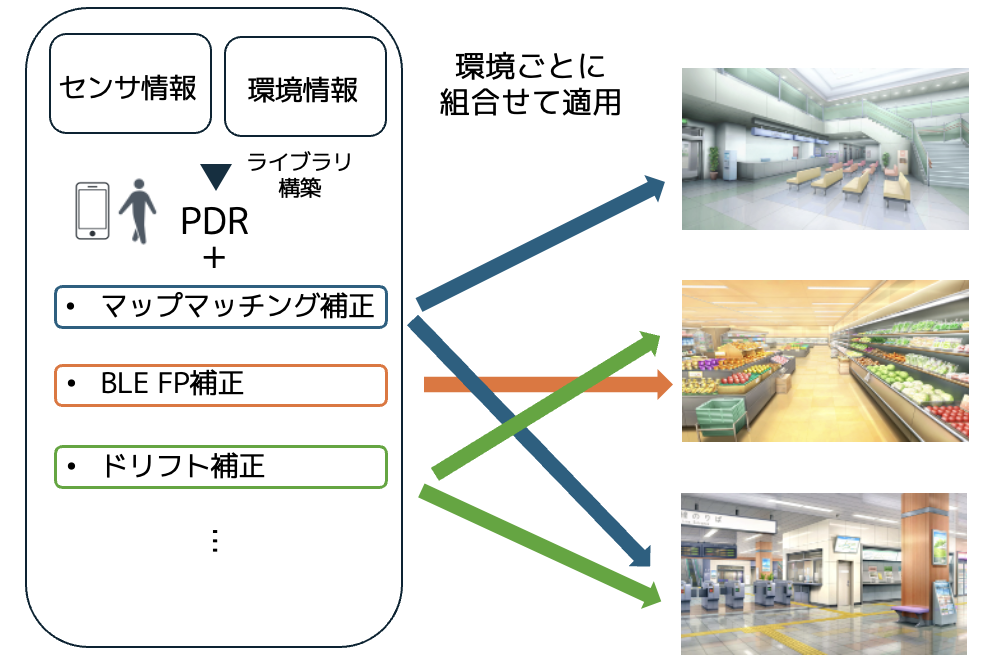
\includegraphics[width=\linewidth]{image/first.png}
	\caption{様々な環境や状況に対応できるPDRベースの\\3次元屋内位置推定ライブラリの概要}    \label{fig:overview}
\end{figure}


\section{PDRベースの3次元屋内位置推定ライブラリの検討}

% 本章では,屋内位置推定ライブラリの基本設計と実装について述べる.
% まず2.1節で要求仕様を整理し,2.2節でxDR Challenge環境における平面的な位置推定について説明する.
% 続いて2.3節では気圧センサを活用した3次元的な位置推定手法について述べる.
% 図2に本ライブラリにおける環境条件に応じた補正の適用例を示す.

\subsection{要求仕様}
屋内環境における位置推定システムの開発には,
環境条件と利用可能な補正情報の多様性を考慮する必要がある.
本ライブラリでは,まず基本となるセンサ情報として,
スマートフォンに搭載された加速度センサとジャイロセンサをPDRの基本処理に利用する.
また気圧センサは階層判定による3次元位置推定を実現する重要な情報源となる.
次に環境情報として,フロアマップ情報とBLEビーコンからの電波強度情報を活用する.
フロアマップは歩行可能な領域の制約として機能し,
PDRの累積誤差を抑制する.BLEビーコンは必要に応じて追加設置が可能であり,
位置推定の補正に柔軟に活用できる.
システムの設計においては,拡張性と環境変化への対応を重視する.
補正アルゴリズムは独立したモジュールとして実装し,
環境に応じて適切な組み合わせが可能な設計とする.
また,特定の補正情報が利用できない状況でも,
基本的なPDR処理は継続して機能する堅牢性を確保する.




\subsection{xDR challengeにおける平面的な位置推定}

本ライブラリの検証として,PDRベンチマーク標準化委員会が主催するxDR Challenge 2023の環境を用いた.このコンテストでは,高速道路のサービスエリアを対象とし,被験者がスマートフォンとハンドヘルドLiDARを保持して歩行する.スマートフォンからは加速度,角速度,地磁気のセンサデータと,各BLEビーコンの受信電波強度が取得される.LiDARからは正確な歩行軌跡が取得され,これを正解データとして扱う.

PDRによる初期推定では,加速度の大きさから歩行タイミングを検出し,角速度の積分により進行方向を推定する.加速度波形に対して適応的な閾値処理を適用することで,歩行者の状態変化に追従しながら安定した歩行検出を実現している.また進行方向の推定では,角速度の積分による累積誤差を考慮し,線形ドリフト補正を導入している.

これらの初期推定に対し,本ライブラリは図3に示すような段階的な補正処理を適用する.補正処理の中核となるTrajectoryCorrectroクラスは,DriftCorrector,MapMatchCorrector,WirelessSignalCorrectorの3つの補正クラスを統合的に管理する.各補正クラスは特定の補正機能を担当し,TrajectoryCorrectorsBuilderを介して柔軟な組み合わせを可能としている.

具体的な補正処理として,まずDriftCorrectorによりジャイロセンサの累積誤差を低減する.この処理では既知の座標との誤差を最小化するドリフト値を探索し,角速度データを補正する.次にMapMatchCorrectorを用いて,フロアマップの構造的特徴から初期進行方向を補正する.この手法は建物の主軸に沿った移動が多いという特徴を利用し,x軸とy軸に対して平行な成分が最大となる方向を探索する.さらに,歩行可能領域の情報を用いて最適な進行方向を決定する.

WirelessSignalCorrectorでは,BLEビーコンの受信強度情報を用いた2つの補正アプローチを提供する.一つは送信機の基地局位置を既知とし,受信強度の閾値処理と距離の最適化により軌跡を補正する手法である.もう一つはフィンガープリントを用いた手法で,事前に収集した電波強度パターンと実測値の類似度に基づいて位置を推定する.特に基地局位置が未知の環境でも適用可能という利点を持つ.

図4に初期推定軌跡,正解軌跡,最終補正後の推定軌跡を示す.初期進行方向の誤差とドリフトによる軌跡の歪みが,段階的な補正により大幅に改善されているのが確認できる.また,補正後の軌跡は建物の構造とも良く整合している.

% TODO: 背景消したいけどremove.bgすると文字の解像度が落ちる.
% 後ベクター画像になるべくしたい
\begin{figure}[h]
    \centering
    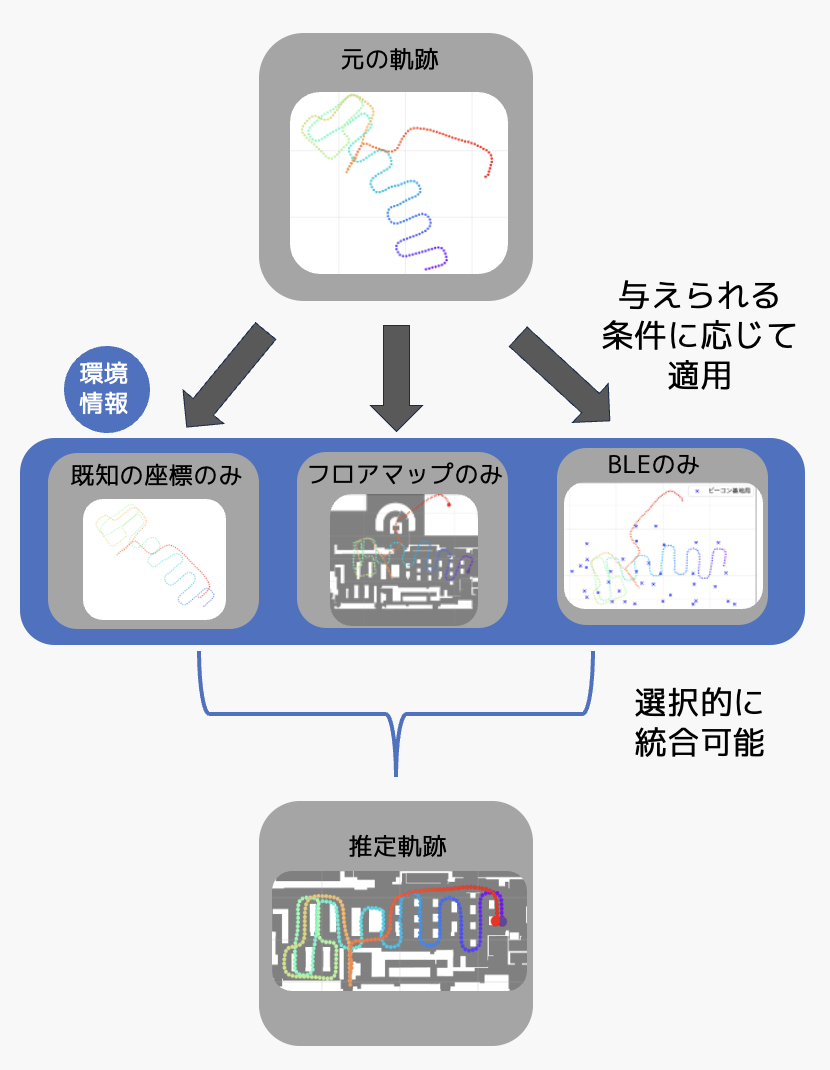
\includegraphics[width=\linewidth]{image/integrate4.jpg}
    \caption{環境条件に応じた補正の適用}
    \label{fig:corrector-class}
\end{figure}


\subsection{気圧データを用いた3次元的な位置推定}

屋内環境における3次元的な位置推定において,ユーザの階層の把握は重要な課題である.本ライブラリではスマートフォンの気圧センサから得られるデータを活用し,PDRによる2次元軌跡に階層情報を付加する手法を実装している.

気圧データを用いた階層検知には,センサ自体のノイズや量子化誤差による変動,気象条件による外気圧の変動,エレベーターや階段移動時の急激な気圧変化,さらに建物内の空調システムによる局所的な気圧変化といった課題が存在する.これらの課題に対処するため,本ライブラリでは安定区間検出とクラスタリングを組み合わせた2段階の手法を採用している.

図5に示すように,まず気圧の安定区間を検出する.ここでは気圧変動の閾値として0.02 hPa(約1.7mの高度差に相当)と,最小継続時間として4秒というパラメータを用いる.次に検出された安定区間内の気圧値に対してDBSCANアルゴリズムを適用し,階層のグルーピングを行う.DBSCANのパラメータは,標準大気圧の高度による変化(約12 Pa/m)と標準的な階高(3.0 m)を考慮して設定する.

階層間の遷移は,安定区間の間に観測される顕著な気圧変化として検出される.本手法では,連続する安定区間の間の気圧の変化パターンを分析することで,エレベーターや階段による移動を検知する.これにより,商業施設やオフィスビルなど,複数階層を有する建物内での継続的な位置推定を実現している.


\section{評価と他環境での検討}









\subsection{xDR Challenge 2023 環境での評価}

本ライブラリの評価として,xDR Challenge 2023の評価フレームワークを用いた検証を行った.
このフレームワークでは,円形誤差(l\_ce),局所空間における円形精度(l\_ca),誤差蓄積勾配(l\_eag),速度誤差(l\_ve),障害物回避要件(l\_obstacle)の5つの評価指標が用いられる.

評価結果では,l\_ce(88.55),l\_eag(93.02),l\_ve(95.55),l\_obstacle(93.48)において一定の精度を達成した.
特に速度誤差と障害物回避要件で95前後の高いスコアを記録し,
基本的なPDRアルゴリズムとフロアマップの補正が効果的に機能していることが示された.
一方,局所空間における円形精度(l\_ca)は62.51と低い結果となった.これは実装アルゴリズムが比較的シンプルな構成であり,環境変化への対応力が限定的であることを示唆している.



\subsection{他環境での検討}

本ライブラリの他環境への適用可能性として,駅構内と大学キャンパスでの検討を行った.
駅構内では,改札の位置を利用したドリフト補正が有効である.
改札は固定位置であり,ICカードの利用により通過時刻が正確に記録できる特徴を持つ.
また,フロアマップ情報も入手しやすく,マップマッチング補正の適用が期待できる.

大学キャンパスでは,Wi-Fiの基地局を活用した補正が有効である.
キャンパス内の各建物には基本的にWi-Fi基地局が設置されており,
BLEビーコンの新規設置に比べて導入コストを抑えられる.
ただし,基地局の正確な位置情報の把握は困難な場合が多いため,
フィンガープリント方式の補正が適している.
また,研究室やサークルなど異なるコミュニティが混在する環境では,
各コミュニティへの機器設置の申請コストなども考慮する必要がある.

\section{今後の課題}

PDRアルゴリズムの基本性能の向上は,引き続き重要な課題である.
現状の実装では,歩行タイミングの検出に適応的な閾値処理を用いているが,
歩行速度や路面状況の急激な変化に対する追従性には改善の余地がある.
また,方向推定においては地磁気センサとの融合による補正が考えられるが,磁場の歪みが大きい環境での安定性確保が技術的な課題となる.

システム設計面では,処理の優先順位付けや条件分岐の制御についての改善が必要である.
現在のビルダーパターンによる設計は補正処理の柔軟な組み合わせを可能としているが,
環境条件の変化に応じた動的な処理の切り替えには対応していない.
また,リアルタイムでの位置推定を実現するため,
センサーデータの非同期処理への対応も課題となる.

評価方法の拡充も重要である.xDR Challenge 2023の環境での評価に加え,
商業施設やオフィスビル,地下街など,
異なる特性を持つ環境での検証を進める必要がある.
また,センサーの経年劣化や環境の季節変化など,
長期運用時の安定性に関する評価も重要な課題である.

% 課題としてPDRアルゴリズムの基本性能の向上が挙げられる.
% 現状の実装では,歩行タイミングの検出に適応的な閾値処理を用いているが,
% 歩行速度や路面状況の急激な変化に対する追従性の改善の余地がある.
% また,方向推定においては地磁気センサとの融合による補正が考えられるが,
% 磁場の歪みが大きい環境での安定性確保が技術的な課題となる.
% さらに,商業施設やオフィスビル,地下街など,異なる特性を持つ環境での検証を進める必要がある.


\bibliographystyle{junsrt}
\bibliography{reference}

\end{document}
